%%%%%%%%%%%%%%%%%%%%%%%% editor.tex %%%%%%%%%%%%%%%%%%%%%%%%%%%%%
%
% sample root file for the contributions of a "contributed volume"
%
% Use this file as a template for your own input.
%
%%%%%%%%%%%%%%%%%%%%%%%%%%%%% Springer %%%%%%%%%%%%%%%%%%%%%%%%%%


% RECOMMENDED %%%%%%%%%%%%%%%%%%%%%%%%%%%%%%%%%%%%%%%%%%%%%%%%%%%
\documentclass[graybox, envcountchap, twocolumn]{styles/svmult}

% general metadata:
\author{soulmachine@gmail.com}
\title{Machine Learning Cheat Sheet}
\subtitle{Classical equations, diagrams and tricks in machine learning}

% choose options for [] as required from the list
% in the Reference Guide

\usepackage{amssymb,amsmath,bm}
\DeclareMathAlphabet{\mathcal}{OMS}{cmsy}{m}{n}
\usepackage{textcomp}
\newcommand\abs[1]{\left\lvert#1\right\rvert}
\usepackage{longtable}
\usepackage{algorithm2e}
\usepackage{tocbibind}
\usepackage[toc]{multitoc}
\usepackage{tabularx}
\renewcommand{\bibname}{References}
\usepackage{mathptmx}        % selects Times Roman as basic font
\usepackage{helvet}          % selects Helvetica as sans-serif font
\usepackage{courier}         % selects Courier as typewriter font
%\usepackage{type1cm}        % activate if the above 3 fonts are 
                             % not available on your system

\usepackage{makeidx}         % allows index generation
\usepackage{graphicx}        % standard LaTeX graphics tool
                             % when including figure files
\usepackage[justification=centering]{caption}
\usepackage{subfig}
\usepackage{multicol}        % used for the two-column index
\usepackage{multirow}
\usepackage[bottom]{footmisc}% places footnotes at page bottom
\usepackage[bookmarksnumbered=true,
            bookmarksopen=true,
            colorlinks=true,
            linkcolor=blue,
            anchorcolor=blue,
            citecolor=blue
           ]{hyperref}

\graphicspath{{figures/}}

% see the list of further useful packages in the Reference Guide

\makeindex             % used for the subject index
                       % please use the style svind.ist with
                       % your makeindex program

%%%%%%%%%%%%%%%%%%%%%%%%%%%%%%%%%%%%%%%%%%%%%%%%%%%%%%%%%%%%%%%%%

\begin{document}

\frontmatter%%%%%%%%%%%%%%%%%%%%%%%%%%%%%%%%%%%%%%%%%%%%%%%%%%%%%%

\include{titlepage}
%\include{dedic}
%\include{foreword}
\include{preface}
%\include{acknow}

\tableofcontents
\include{cblist}
%\include{acronym}
\include{notation}


\mainmatter%%%%%%%%%%%%%%%%%%%%%%%%%%%%%%%%%%%%%%%%%%%%%%%%%%%%%%%
%\include{part}
\include{chapterIntroduction}
\include{chapterProbability}
\include{chapterGenerativeModels}
\include{chapterMVN}
\include{chapterBayesianStatistics}
\include{chapterFrequentistStatistics}
\chapter{Linear Regression}


\section{Introduction}
Linear regression is the “work horse” of statistics and (supervised) machine learning. When augmented with kernels or other forms of basis function expansion, it can model also nonlinear relationships. And when the Gaussian output is replaced with a Bernoulli or multinoulli distribution, it can be used for classification, as we will see below. So it pays to study this model in detail.


\section{Representation}

\begin{equation}
p(y|\vec{x},\vec{\theta})=\mathcal{N}(y|\vec{w}^T\vec{x}, \sigma^2)
\end{equation}
where $\vec{w}$ and $\vec{x}$ are extended vectors, $\vec{x}=(1,x)$, $\vec{w}=(b,w)$.

Linear regression can be made to model non-linear relationships by replacing $\vec{x}$ with some non-linear function of the inputs, $\phi(\vec{x})$ \begin{equation}
p(y|\vec{x},\vec{\theta})=\mathcal{N}(y|\vec{w}^T\phi(\vec{x}), \sigma^2)
\end{equation}

This is known as \textbf{basis function expansion}. (Note that the model is still linear in the parameters $\vec{w}$, so it is still called linear regression; the importance of this will become clear below.) A simple example are polynomial basis functions, where the model has the form
\begin{equation}
\phi(x)=(1, x, \cdots, x^d)
\end{equation}



\section{MLE}
Instead of maximizing the log-likelihood, we can equivalently minimize the \textbf{negative log likelihood} or \textbf{NLL}:
\begin{equation}
\text{NLL}(\vec{\theta}) \triangleq -\ell(\vec{\theta})=-\log(\mathcal{D}|\vec{\theta})
\end{equation}

The NLL formulation is sometimes more convenient, since many optimization software packages are designed to find the minima of functions, rather than maxima.

Now let us apply the method of MLE to the linear regression setting. Inserting the definition of the Gaussian into the above, we find that the log likelihood is given by
\begin{align}
\ell(\vec{\theta})& =\sum\limits_{i=1}^N \log\left[\dfrac{1}{\sqrt{2\pi}\sigma}\exp\left(-\dfrac{1}{2\sigma^2}(y_i-\vec{w}^T\vec{x}_i)^2\right)\right] \\
     & =-\dfrac{1}{2\sigma^2}\text{RSS}(\vec{w})-\dfrac{N}{2}\log(2\pi\sigma^2)
\end{align}

RSS stands for \textbf{residual sum of squares} and is defined by
\begin{equation}
\text{RSS}(\vec{w}) \triangleq \sum\limits_{i=1}^N (y_i-\vec{w}^T\vec{x}_i)^2
\end{equation}

We see that the MLE for $\vec{w}$ is the one that minimizes the RSS, so this method is known as \textbf{least squares}.

Let's drop constants wrt $\vec{w}$ and NLL can be written as
\begin{equation}
\text{NLL}(\vec{w}) = \dfrac{1}{2}\sum\limits_{i=1}^N (y_i-\vec{w}^T\vec{x}_i)^2
\end{equation}

There two ways to minimize NLL$(\vec{w})$.


\subsection{OLS}
Define $\vec{y}=(y_1,y_2,\cdots,y_N)$, $\vec{X}=\left(\begin{array}{c}\vec{x}_1^T \\ \vec{x}_2^T \\ \vdots \\ \vec{x}_N^T\end{array}\right)$, then NLL$(\vec{w})$ can be written as
\begin{equation}
\text{NLL}(\vec{w})=\dfrac{1}{2}(\vec{y}-\vec{X}\vec{w})^T(\vec{y}-\vec{X}\vec{w})
\end{equation}

When $\mathcal{D}$ is small(for example, $N < 1000$), we can use the following equation to compute \vec{w} directly
\begin{equation}
\hat{\vec{w}}_{\mathrm{OLS}}=(\vec{X}^T\vec{X})^{-1}\vec{X}^T\vec{y}
\end{equation}

The corresponding solution $\hat{\vec{w}}_{\mathrm{OLS}}$ to this linear system of equations is called the \textbf{ordinary least squares} or \textbf{OLS} solution.

\begin{proof}
We now state without proof some facts of matrix derivatives (we won’t need all of these at this section).
\begin{eqnarray}
trA &\triangleq& \sum\limits_{i=1}^n A_{ii} \nonumber \\
\frac{\partial}{\partial A}AB &=& B^T \\
\frac{\partial}{\partial A^T}f(A) &=& \left[\frac{\partial}{\partial A}f(A)\right]^T \label{eqn:matrix-1} \\
\frac{\partial}{\partial A}ABA^TC &=& CAB+C^TAB^T \label{eqn:matrix-2} \\
\frac{\partial}{\partial A}|A| &=& |A|(A^{-1})^T
\end{eqnarray}

Then,
\begin{eqnarray*}
\text{NLL}(\vec{w}) &=& \frac{1}{2N}(\vec{X}\vec{w}-\vec{y})^T(\vec{X}\vec{w}-\vec{y}) \\
\frac{\partial \text{NLL}}{\vec{w}} &=& \frac{1}{2} \frac{\partial}{\vec{w}} (\vec{w}^T\vec{X}^T\vec{X}\vec{w}-\vec{w}^T\vec{X}^T\vec{y}-\vec{y}^T\vec{X}\vec{w}+\vec{y}^T\vec{y}) \\
                           &=& \frac{1}{2} \frac{\partial}{\vec{w}} (\vec{w}^T\vec{X}^T\vec{X}\vec{w}-\vec{w}^T\vec{X}^T\vec{y}-\vec{y}^T\vec{X}\vec{w}) \\
						   &=& \frac{1}{2} \frac{\partial}{\vec{w}} tr(\vec{w}^T\vec{X}^T\vec{X}\vec{w}-\vec{w}^T\vec{X}^T\vec{y}-\vec{y}^T\vec{X}\vec{w}) \\
						   &=& \frac{1}{2} \frac{\partial}{\vec{w}} (tr\vec{w}^T\vec{X}^T\vec{X}\vec{w}-2tr\vec{y}^T\vec{X}\vec{w})
\end{eqnarray*}

Combining Equations \ref{eqn:matrix-1} and \ref{eqn:matrix-2}, we find that 
\begin{equation*}
\frac{\partial}{\partial A^T}ABA^TC = B^TA^TC^T+BA^TC
\end{equation*}

Let $A^T=\vec{w}, B=B^T=\vec{X}^T\vec{X}$, and $C=I$, Hence,
\begin{eqnarray}
\frac{\partial \text{NLL}}{\vec{w}} &=& \frac{1}{2} (\vec{X}^T\vec{X}\vec{w}+\vec{X}^T\vec{X}\vec{w} -2\vec{X}^T\vec{y}) \nonumber \\
						   &=& \frac{1}{2} (\vec{X}^T\vec{X}\vec{w} - \vec{X}^T\vec{y}) \nonumber \\
\frac{\partial \text{NLL}}{\vec{w}} &=& 0 \Rightarrow \vec{X}^T\vec{X}\vec{w} - \vec{X}^T\vec{y} =0 \nonumber \\
\vec{X}^T\vec{X}\vec{w} &=& \vec{X}^T\vec{y} \label{eqn:normal-equation} \\
\hat{\vec{w}}_{\mathrm{OLS}} &=& (\vec{X}^T\vec{X})^{-1}\vec{X}^T\vec{y} \nonumber
\end{eqnarray}
\end{proof}

Equation \ref{eqn:normal-equation} is known as the \textbf{normal equation}.


\subsubsection{Geometric interpretation}

See Figure \ref{fig:graphical-interpretation-of-OLS}.
\begin{figure}[hbtp]
\centering
    \includegraphics[scale=.50]{graphical-interpretation-of-OLS.png}
\caption{Graphical interpretation of least squares for $N=3$ examples and $D=2$ features. $\tilde{\vec{x}}_1$ and $\tilde{\vec{x}}_2$˜ are vectors in $\mathbb{R}^3$; together they define a 2D plane. $\vec{y}$ is also a vector in $\mathbb{R}^3$ but does not lie on this 2D plane. The orthogonal projection of $\vec{y}$ onto this plane is denoted $\hat{\vec{y}}$. The red line from $\vec{y}$ to $\hat{\vec{y}}$ is the residual, whose norm we want to minimize. For visual clarity, all vectors have been converted to unit norm.}
\label{fig:graphical-interpretation-of-OLS} 
\end{figure}

To minimize the norm of the residual, $\vec{y}-\hat{\vec{y}}$, we want the residual vector to be orthogonal to every column of $\vec{X}$,so˜ $\tilde{\vec{x}}_j(\vec{y}-\hat{\vec{y}})=0$ for $j=1:D$. Hence
\begin{equation}\begin{split}
\tilde{\vec{x}}_j(\vec{y}-\hat{\vec{y}})=0 & \Rightarrow \vec{X}^T(\vec{y}-\vec{X}\vec{w})=0 \\
                                           & \Rightarrow \vec{w}=(\vec{X}^T\vec{X})^{-1}\vec{X}^T\vec{y}
\end{split}\end{equation}


\subsection{SGD}
When $\mathcal{D}$ is large, use stochastic gradient descent(SGD).

\begin{align}
\because \dfrac{\partial}{\partial w_i}\text{NLL}(\vec{w})=& \sum\limits_{i=1}^N (\vec{w}^T\vec{x}_i-y_i)x_{ij} \\
\therefore w_j=& w_j - \alpha\dfrac{\partial}{\partial w_j}\text{NLL}(\vec{w}) \nonumber \\
                  =& w_j - \sum\limits_{i=1}^N \alpha(\vec{w}^T\vec{x}_i-y_i)x_{ij} \\
\therefore \vec{w}=& \vec{w}-\alpha(\vec{w}^T\vec{x}_i-y_i)\vec{x}
\end{align}


\section{Ridge regression(MAP)}
One problem with ML estimation is that it can result in overfitting. In this section, we discuss a way to ameliorate this problem by using MAP estimation with a Gaussian prior.


\subsection{Basic idea}
We can encourage the parameters to be small, thus resulting in a smoother curve, by using a zero-mean Gaussian prior:
\begin{equation}
p(\vec{w})=\prod\limits_j \mathcal{N}(w_j|0,\tau^2)
\end{equation}
where $1/\tau^2$ controls the strength of the prior. The corresponding MAP estimation problem becomes
\begin{equation}
\arg\max_{\vec{w}} \sum\limits_{i=1}^N \log{\mathcal{N}(y_i|w_0+\vec{w}^T\vec{x}_i,\sigma^2)}+\sum\limits_{j=1}^D \log{\mathcal{N}(w_j|0,\tau^2)}
\end{equation}

It is a simple exercise to show that this is equivalent to minimizing the following
\begin{equation}\label{eqn:Ridge-regression-J}
J(\vec{w})=\dfrac{1}{N}\sum\limits_{i=1}^N (y_i-(w_0+\vec{w}^T\vec{x}_i))^2+\lambda\lVert\vec{w}\rVert^2 , \lambda \triangleq \dfrac{\sigma^2}{\tau^2}
\end{equation}

Here the first term is the MSE/ NLL as usual, and the second term, $\lambda \geq 0$, is a complexity penalty. The corresponding solution is given by
\begin{equation}\label{eqn:Ridge-regression-solution}
\hat{\vec{w}}_{\mathrm{ridge}}=(\lambda\vec{I}_D+\vec{X}^T\vec{X})^{-1}\vec{X}^T\vec{y}
\end{equation}

This technique is known as \textbf{ridge regression},or \textbf{penalized least squares}. In general, adding a Gaussian prior to the parameters of a model to encourage them to be small is called $\ell_2$ \textbf{regularization} or \textbf{weight decay}. Note that the offset term $w_0$ is not regularized, since this just affects the height of the function, not its complexity.

We will consider a variety of different priors in this book. Each of these corresponds to a different form of \textbf{regularization}. This technique is very widely used to prevent overfitting.


\subsection{Numerically stable computation *}

\begin{equation}\label{eqn:Ridge-regression-SVD}
\hat{\vec{w}}_{\mathrm{ridge}}=\vec{V}(\vec{Z}^T\vec{Z}+\lambda\vec{I}_N)^{-1}\vec{Z}^T\vec{y}
\end{equation}


\subsection{Connection with PCA *}


\subsection{Regularization effects of big data}
Regularization is the most common way to avoid overfitting. However, another effective approach — which is not always available — is to use lots of data. It should be intuitively obvious that the more training data we have, the better we will be able to learn.

In domains with lots of data, simple methods can work surprisingly well (Halevy et al. 2009). However, there are still reasons to study more sophisticated learning methods, because there will always be problems for which we have little data. For example, even in such a data-rich domain as web search, as soon as we want to start personalizing the results, the amount of data available for any given user starts to look small again (relative to the complexity of the problem).


\section{Bayesian linear regression}
TODO

\section{Linear Regression Diagnostic}

Considering the linear model \(y = X_{n \times p}\beta_{p} + \epsilon\),
and its commonly used estimator OLSE:
\(\hat{\beta} = \ (X^{\top}X)^{- 1}X^{\top}y\).

There several common (linear) regression diagnostic need to be done:

\begin{enumerate}
	\def\labelenumi{\arabic{enumi}.}
	\item
	Unusual and influential data, Outliers
	\item
	Normality
	\item
	Nonconstant error of variance
	\item
	Multicollinearity
	\item
	Non-linearity
	\item
	Model Specification
	\item
	Independence
\end{enumerate}

\subsection{Unusual and influential data,
	Outliers}\label{unusual-and-influential-data-outliers}

\begin{enumerate}
	\def\labelenumi{\alph{enumi}.}
	\item
	What is \textbf{influential point}? Howto detect?
	\item
	What is \textbf{outliers}? Howto detect?
\end{enumerate}

\begin{figure}\centering
	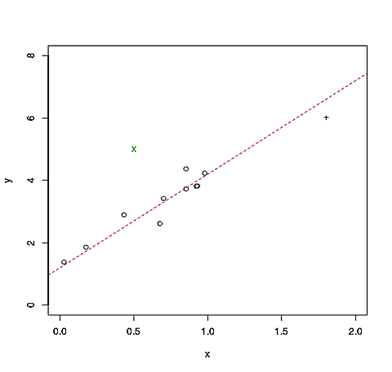
\includegraphics[scale=.6]{./figures/lm_ivo.png}
	\caption{Influential v.s. outliers}
\end{figure}

In short, we summarize the distinction between these two concepts as
follows:

\begin{itemize}
	\item
	A data point is \textbf{influential} if it unduly \emph{influences any
		part of a regression analysis}, such as the predicted responses, the
	estimated slope coefficients, or the hypothesis test results.
	(\textbf{+}) changes \(R^{2}\), \emph{P}-value, \ldots{}
	\item
	An \textbf{outlier} is a data point whose response
	\emph{\textbf{y}}\footnote{In many cases, one could also define
		outliers corresponding to \emph{\textbf{X}} instead of
		\emph{\textbf{y}}.} does not follow the \emph{general trend of the
		rest of the data}. (\textbf{x})
\end{itemize}

An easy way to determine if the data point is influential is to find the
best fitting line twice --- once with the given data point included and
once the given data point excluded. Formally, \textbf{leverage}
statistics could be used to identify extreme values.

Denote the projection matrix \emph{H} as \(X(X^{\top}X)^{- 1}X^{\top}\),
and we could indeed rewrite the prediction
into\(\hat{y_{}} = X\hat{\beta} = H\ y\), which clearly indicates that
the prediction is a \emph{linear combination} of observed y. This is
also the reason why it is called regression. Besides, one may also
notice that the i-th prediction is determined by the i-th row of the
projection matrix. Leverage is defined as the i-i th entry of the
projection matrix, i.e. \(H_{\text{ii}}\), and as it is called, could
somewhat determine the value of the i-th prediction value( as
\({\hat{y}}_{i} = H_{i}\text{\ y}\)). Some linear algebra shows

\begin{itemize}
	\item
	\(trace(H)\  = sum\ of\ eigen\ value = \ p\  = \ \sum_{i = 1}^{n}H_{\text{ii}}\)
	\item
	As H is the projection matrix (H\textgreater{}0 and orthogonal),
	\textbf{leverage} is always in range {[}0,1{]} \footnote{Every entry
		of an orthogonal matrix must be between 0 and 1, as the L2 norm of
		any row/column =1}
	\item
	The leverage \(H_{\text{ii}}\) is a measure of the distance between
	the X value for the i-th data point and the mean of the X values for
	all n data points.
\end{itemize}

\noindent\textbf{General rule: 3 times rule}

If
\(H_{\text{ii}} > 3\frac{p}{n} = 3\frac{1}{n}\sum_{i = 1}^{n}H_{\text{ii}}\)
, then we say `` we could identify x values that are \textbf{extreme}
and therefore \textbf{potentially influential} on our regression
analysis.''

Also, there are other summary statistics, eg: studentized residual($t_i=\frac{\hat{\epsilon}_i}{\hat{\sigma}\sqrt{1-h_{ii}}}$),
Cook's D, DFFITS( studentized residual times
$\sqrt{h_{ii}/(1-h_{ii})}$
and DFBETAs(Thumb of rule: \(2/\sqrt{n}\)).

\subsection{Normality}\label{normality}

It is often not critical but helpful to set the normal assumption in
linear regression. Normality offers a way to \textbf{test} whether the
coefficients were 0. Please notice that we could still use OLSE without
normal assumption to \textbf{estimate}\(\hat{\beta}\)when NO HYPOTHESIS
TESTING IS NEEDED.

\begin{itemize}
	\item
	QQ Plot (of residual);
	\item
	KS test among many others (e.g. the Kolmogorov-Smirnov test, the
	Shapiro-Wilk test, the Jarque-Bera test, and the
	\textbf{Anderson-Darling test}\footnote{Most used one.}).
\end{itemize}

The causes of non-normality varies, eg.

\begin{enumerate}
	\def\labelenumi{\alph{enumi}.}
	\item
	The prediction error (\textbf{NOT X!!!!}) is not normal;
	\item
	the data is not linearly constructed/not additive(e.g. y=x1*x2 or
	x1*x1);
	\item
	there are several subgroups in the data that have different
	statistical properties.
\end{enumerate}

\subsection{Nonconstant error of
	variance}\label{nonconstant-error-of-variance}

One important note first: OLS is still the unbiased estimator but not
the BLUE(best unbiased linear estimator for \(c^{\top}y\)).

\emph{Proof}:

\begin{enumerate}
	\def\labelenumi{\arabic{enumi}.}
	\item
	unbiased estimator:
	\(E\lbrack\hat{\beta}\rbrack = E\lbrack\ (X^{\top}X)^{- 1}X^{\top}y\rbrack = E\lbrack\ (X^{\top}X)^{- 1}X^{\top}(X\beta + \epsilon)\rbrack = \beta\ \)
	\item
	not BLUE: Assume \(\epsilon \sim N(0,\Sigma)\), we typically could use
	the updated model:
	\(y' = \Sigma^{- \frac{1}{2}}y = x'\beta + \epsilon' = \Sigma^{- \frac{1}{2}}X_{n \times p}\beta_{p} + \Sigma^{- \frac{1}{2}}\epsilon\),
	hence BLUE is OLSE for the updated model. Another way to interpret
	this is MLE. MLE, with the normal assumption, could be finally
	simplify to a weighted least square, which is exactly same as previous
	result. \textbf{QED}
\end{enumerate}

It is also call violence of \textbf{homoscedasticity of variances/heteroscedasticity}. Most of time, one could read this through
\emph{\textbf{(adjusted) residuals vs predicted values}} or even vs
variables.

If one does find any heteroscedasticity, variance stabilizing
transformation could be used, such as Box-Cox transformation\footnote{Box-Cox
	is often used to deal with normality( SAS \textbf{PROC} TRANSREG)} and
more. The reason is simply:

\(Var(f(x))\  \simeq f'(\mu)Var(X)\).

Remember that: in order to perform hypothesis testing on transformed
data, we need to use Delta method again to get the Wald-Confidence
interval.

\emph{Useful tips}

\begin{quote}
	z = sqrt(count); /* \textbf{counts} (\emph{Poisson distribution}) */\\
	/* variance proportional to mean */
	
	z = log(conc); /* concentrations, weights (log normal) */\\
	/* SD proportional to mean */\\
	/* \emph{constant coefficient} of variation (CV) */
	
	z = arsin(sqrt(prop));/* \textbf{proportions} (0-1) */
	
	z = arsin(sqrt(pct/100));/* \textbf{percentages} (0-100) */\\
	/* (\emph{Binomial distribution}) */\\
	/* variance proportional highest in middle*/
\end{quote}

A special case: the equality of variances for a variable calculated for
two or more group

Please read
\href{https://en.wikipedia.org/wiki/Levene\%27s_test}{\emph{Levene's
		test}}, Bartlett's Test and Brown--Forsythe test.

\subsection{Multicollinearity}\label{multicollinearity}

Multicollinearity is a statistical phenomenon that is commonly seen in
linear model. Strictly speaking, it means a perfect linear relationship
among explanatory variables, i.e. \(rank(X) < min(n,p)\).

Considering the estimation equation of LM:
\(\hat{\beta} = (X^{\top}X)^{- 1}X^{\top}Y\),\footnote{One can still use
	Moore--Penrose pseudoinverse or other pseudo-inverse (- or + inverse)
	to get the BLUE.} and hence \(SE(\hat{\beta})\) if the matrix is not
full rank, then the estimation has:

\emph{\textbf{\emph{Cons}}}

\begin{enumerate}
	\def\labelenumi{\arabic{enumi}.}
	\item
	Multicollinearity inflates the variances of the parameter estimates
	and hence this may lead to lack of statistical significance of
	individual predictor variables even though the overall model may be
	significant.
	\item
	The presence of multicollinearity can cause serious problems with the
	estimation of \(\beta\) and the interpretation.
\end{enumerate}

\subsubsection{Detection}\label{detection}

\begin{enumerate}
	\def\labelenumi{\arabic{enumi}.}
	\item
	\textbf{Examination of Correlation Matrix}: Large correlation
	coefficients in the correlation matrix of predictor variables indicate
	multicollinearity. If there is a multicollinearity between any two
	predictor variables, then the correlation coefficient between these
	two variables will be near to unity.
	\item
	\textbf{Variance Inflation Factor (VIF)}: j-VIF is defined as the
	\(\frac{1}{1 - {R_{j}}^{2}}\), where \({R_{j}}^{2}\)denotes the
	\emph{coefficient of determination}\footnote{coefficient of
		determination is \textbf{SS}res/\textbf{SS}total} when
	\(X_{j} \sim X_{- j}\). Rule of Thumb: If \textbf{VIF
		\textgreater{}5,10}\footnote{Montgomery, Douglas C., and Douglas C.
		Montgomery. \emph{Design and analysis of experiments}. Vol. 7. New
		York: Wiley, 1984.}, then we say the multicollinearity is heavy.
	\item
	\textbf{Eigensystem Analysis of Correlation Matrix}: eigensystem plays
	an essential role in regression analysis. Rule of Thumb: If one or
	more of the eigenvalues are small (close to zero) and the
	corresponding condition number(\(\lambda_{\max}/\lambda_{j}\)) is
	large, then it indicates multicollinearity.
\end{enumerate}

Indeed, 1 and 3 are equivalent.

\subsubsection{Solution}\label{solution}

Manually select, \textbf{Stepwise} method, \textbf{PLS}, \textbf{PCA},
\textbf{Shrinkage} regression(Ridge/LASSO, etc). Check topic 2(Linear
Model Extension) for reference.

For stepwise, we need to pay attention to AIC/BIC criterion\footnote{Modifying
	comments from Dr Runze
	Li:\href{https://methodology.psu.edu/media/techreports/12-119.pdf}{\emph{https://methodology.psu.edu/media/techreports/12-119.pdf}}},
they are both \textbf{penalized-likelihood criteria}. They are sometimes
used for \textbf{choosing best predictor subsets in regression} and
often used for comparing non-nested models, which ordinary statistical
tests cannot do. The AIC or BIC for a model is usually written in the
form \(\mathbf{- 2\ Log\ Lik\  + \ k \times p}\), where \emph{Lik} is
the likelihood function, \emph{p} is the number of parameters in the
model, and

\begin{table}
	\centering
	\begin{tabularx}{.475\textwidth}{|l|l|X|}
		\hline
		\textbf{Model} & \textbf{k} & \textbf{Comment}\\\hline
		AIC & 2 & AIC is an estimate of a \textbf{constant} plus the relative
		distance between the unknown true likelihood function of the data and
		the fitted likelihood function of the model, so that a lower AIC means a
		model is considered to be closer to the truth. \textbf{ALWAYS chooses
			too big a model.}\\
		BIC & kog(n) & BIC is an estimate of a function of the \textbf{posterior
			probability} of a model being true, under a certain Bayesian setup, so
		that a lower BIC means that a model is considered to be more likely to
		be the true model. \textbf{MORE likely than AIC to choose too small a
			model.}\\\hline
	\end{tabularx}
	\caption{AIC BIC short summary.}\label{table::aicbiclm}
\end{table}


Both criteria are based on \textbf{various assumptions and asymptotic
	approximations}. Each, despite its heuristic usefulness, has therefore
been criticized as having questionable validity for real world data. But
despite various subtle theoretical differences, their only difference in
practice is the size of the penalty; BIC penalizes model complexity more
heavily. The only way they should disagree is when \textbf{AIC chooses a
	larger model than BIC}.

AIC and BIC are both approximately correct according to a different goal
and a different set of asymptotic assumptions. Both sets of assumptions
have been criticized as unrealistic. Understanding the difference in
their practical behavior is easiest if we consider the simple case of
comparing two nested models. In such a case, several authors have
pointed out that IC's become equivalent to likelihood ratio tests with
different alpha levels. Checking a chi-squared table, we see that AIC
becomes like a significance test at alpha=.16, and BIC becomes like a
significance test with alpha depending on sample size, e.g., .13 for n =
10, .032 for n = 100, .0086 for n = 1000, .0024 for n = 10000. Remember
that power for any given alpha is increasing in n. Thus, AIC always has
a chance of choosing too big a model, regardless of n. BIC has very
little chance of choosing too big a model if n is sufficient, but it has
a larger chance than AIC, for any given n, of choosing too small a
model.

So what's the bottom line? In general, it might be best to use AIC and
BIC together in model selection. For example, in selecting the number of
latent classes in a model, if BIC points to a three-class model and AIC
points to a five-class model, it makes sense to select from models with
3, 4 and 5 latent classes. AIC is better in situations when a false
negative finding would be considered more misleading than a false
positive, and BIC is better in situations where a false positive is as
misleading as, or more misleading than, a false
negative.

\subsection{Summary}\label{summary}

\begin{enumerate}
	\def\labelenumi{\arabic{enumi}.}
	\item
	Detecting Unusual and Influential Data
	
	\begin{enumerate}
		\def\labelenumii{\alph{enumii}.}
		\item
		scatterplots of the dependent variables versus the independent
		variable
		\item
		looking at the largest values of the studentized residuals,
		leverage, Cook's D, DFFITS and DFBETAs
	\end{enumerate}
	\item
	Tests for Normality of Residuals Tests for Heteroscedasticity
	
	\begin{enumerate}
		\def\labelenumii{\alph{enumii}.}
		\item
		kernel \textbf{density plot (e.g, HIST)}
		\item
		\textbf{q}uantile-\textbf{q}uantile plots
		\item
		Shapiro-Wilk W test/KS test
		\item
		residual plot ( residual versus predicted values )
		\item
		White test
	\end{enumerate}
	\item
	Tests for Multicollinearity
	
	\begin{enumerate}
		\def\labelenumii{\alph{enumii}.}
		\item
		VIF
		\item
		Cov matrix
	\end{enumerate}
	\item
	Tests for Non-Linearity
	
	\begin{enumerate}
		\def\labelenumii{\alph{enumii}.}
		\item
		scatterplot of independent variable versus dependent variable
	\end{enumerate}
	\item
	Tests for Model Specification/Independencies
	
	\begin{enumerate}
		\def\labelenumii{\alph{enumii}.}
		\item
		time series
		\item
		Durbin-Watson test
	\end{enumerate}
	\item
	Test of skewness: use kurtosis
\end{enumerate}

\include{chapterLogisticRegression}
\include{chapterGLM}
\include{chapterDGM}
\include{chapterEM}
\include{chapterLatentLinearModels}
\include{chapterSparseLinearModels}
\include{chapterKernels}
\include{chapterGP}
\include{chapterABM}
\include{chapterHMM}
\include{chapterSSM}
\include{chapterUGM}
\include{chapterExactInferenceForGraphicalModels}
\include{chapterVariationalInference}
\include{chapterMoreVariationalInference}
\include{chapterMonteCarloInference}
\include{chapterMCMC}
\include{chapterClustering}
\include{chapterStructureLearning}
\include{chapterLVM}
\include{chapterDeepLearning}
%

\backmatter%%%%%%%%%%%%%%%%%%%%%%%%%%%%%%%%%%%%%%%%%%%%%%%%%%%%%%%
\appendix
\include{chapterOptimization}
\include{glossary}
\printindex

%%%%%%%%%%%%%%%%%%%%%%%%%%%%%%%%%%%%%%%%%%%%%%%%%%%%%%%%%%%%%%%%%%%%%%

\end{document}

